
%NO PREAMBLE, NO \begin{document} or \usepackage here !
\subsection{Симметрия расщеплений d-орбиталей. Энергия стабилизации кристаллическим полем.}

\subsubsection*{ЭСКП}

Энергия стабилизации кристаллическим полем (ЭСКП) — энергия электронной конфигурации иона переходного металла относительно средней энергии орбиталей. Стабилизация возникает вследствие того, что в поле лигандов энергетический уровень некоторых орбиталей ниже, чем в гипотетическом сферическом поле, в котором на все пять d-орбиталей действует одинаковая сила отталкивания, и все d-орбитали вырождены. Например, в октаэдрическом случае уровень $t_{2g}$ ниже, чем средний уровень в сферическом поле. Следовательно, если в данных орбиталях находятся электроны, то ион металла более стабилен в поле лигандов относительно сферического поля. Наоборот, энергетический уровень орбиталей $e_g$ выше среднего, и электроны, находящиеся в них, уменьшают стабилизацию.


\begin{figure}[H]
\centering
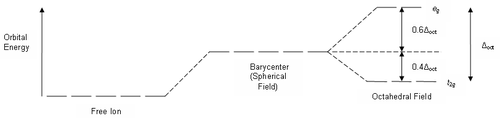
\includegraphics[scale=.750]{/home/someanonimcoder/TeX/tic_summer/images/CFSE.png}
\caption{диарграмма расщепления}
\label{}
\end{figure}

\subsubsection*{Типичные расщепления}

Для получения этих расщеплений обычно рассмтривают изолированные орбитали d, к которым "придвигают" 8 заместителей, получая октаэдрическое расщепление, от которого потом постепенно "убирают" заместители.

\begin{figure}[H]%
    \centering
    \subfloat[катринка]{{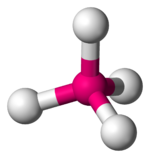
\includegraphics[width=5cm]{images/tetrahedr.png} }}%
    \qquad
    \subfloat[диаграмма орбиталей]{{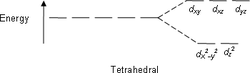
\includegraphics[width=5cm]{images/tetrahedr_orb.png} }}%
    \label{fig:example}%
        \caption{Тетраэдрическое расщепление}
\end{figure}



\begin{figure}[H]%
    \centering
    \subfloat[катринка]{{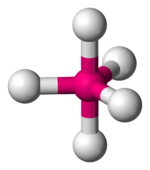
\includegraphics[width=5cm]{images/trig-bip.png} }}%
    \qquad
    \subfloat[диаграмма орбиталей]{{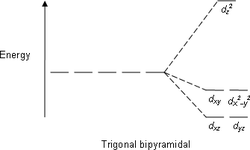
\includegraphics[width=5cm]{images/trig-bip_orb.png} }}%
    \label{fig:example}%
    \caption{Тригонально-бипирамидальное расщепление}
\end{figure}


\begin{figure}[H]%
    \centering
    \subfloat[катринка]{{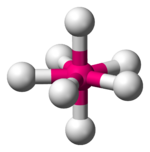
\includegraphics[width=5cm]{images/pent-bip.png} }}%
    \qquad
    \subfloat[диаграмма орбиталей]{{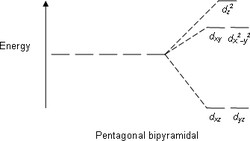
\includegraphics[width=5cm]{images/pent-bip_orb.png} }}%
    \label{fig:example}%
    \caption{Пентагонально-бипирамидальное расщепление}
\end{figure}


\begin{figure}[H]%
    \centering
    \subfloat[катринка]{{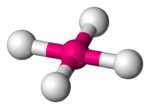
\includegraphics[width=5cm]{images/planar.png} }}%
    \qquad
    \subfloat[диаграмма орбиталей]{{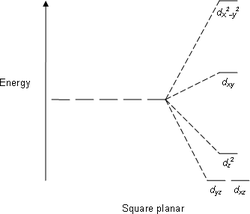
\includegraphics[width=5cm]{images/planar_orb.png} }}%
    \label{fig:example}%
    \caption{Плоскоквадрвтное расщепление}
\end{figure}

\begin{figure}[H]%
    \centering
    \subfloat[катринка]{{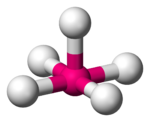
\includegraphics[width=5cm]{images/sq-piram.png} }}%
    \qquad
    \subfloat[диаграмма орбиталей]{{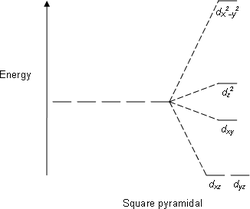
\includegraphics[width=5cm]{images/sq-piram_orb.png} }}%
    \label{fig:example}%
    \caption{Квадратно-пирамидальное расщепление}
\end{figure}

\begin{figure}[H]%
    \centering
    \subfloat[катринка]{{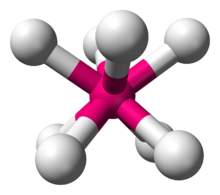
\includegraphics[width=5cm]{images/sq-antipr.png} }}%
    \qquad
    \subfloat[диаграмма орбиталей]{{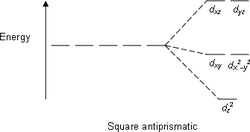
\includegraphics[width=5cm]{images/sq-antipr_orb.png} }}%
    \label{fig:example}%
    \caption{Квадратно-антипризматическое расщепление}
\end{figure}




